\section{Introduction}
Gas phase Electron Diffraction  (GED) is one of only two existing methods for the direct determination of molecular structure parameters in gas phase. Even though the method  was introduced in the 1930th, analysis of the experimental data is not trivial or automated as it is in X-Ray diffraction.\\ 
GED is based on the diffraction of electrons by randomly orientated molecules in the gas phase. The compound is evaporated into high vacuum ($\approx 10^{-7}$ Torr) though a nozzle where an electron beam crosses the molecular jet.\\
The electrons are emitted thermally and accelerated by an electric potential.  The beam is focused by magnetic or electric fields and then guided into the diffraction chamber. The electron beam is well defined in terms of the wavelengths $\lambda$ with a fluctuation not bigger than 0.1 \%. \\
Upon interaction of the electron beam with the molecular jet in the diffraction chamber  several processes may occurs. Because of the low pressure the probability that an electron is not scattered is 99 \%. This directly leads to the reasonable assumption that multiple scattering of one electron can be neglected. \\
For the rest of the electrons scattering occurs.  Neglecting rotational-vibrational coupling, the elastic electron scattering intensity for a molecule with $N$ atoms reads as: 
\begin{equation*}
I(s) = \frac{K^2I_0}{R^2}\left(  \underbrace{\sum_i^N |f_i(s)|^2}_{\textnormal{Atomic scattering}} +  \underbrace{\sum^N_{ \substack{i,j \\ i\neq j}}f_i(s)f_i^*(s) \frac{\sin sr_{ij}}{sr_{ij}}}_{\textnormal{Molecular scattering}} \right)
\end{equation*}
Where $s = 2 k_0 \sin \theta/2$ is the absolute value of the momentum transfer, $\theta$ is the scattering angle, $K$ is a constant, $R$ is the distance of the observation point from the scattering center, $f(s)$ are the electron scattering amplitudes and $r_{ij}$ = $|\vec{r_i}-\vec{r_j}|$ (with $\vec{r_i}$ as the position vector of the atom $i$ in the molecular coordinate system). The atomic scattering is the dominant factor, but its intensity is not relevant to the molecular structure problem since it does not contain any information about the inter-atomic distances.  \\
This model can be expanded to include vibration. In this approximation the molecular scattering intensity reads as: 
\begin{equation*}
I_m(s) = \frac{K^2I_0}{R^2} \sum^N_{ \substack{i,j \\ i\neq j}}g_{ij}(s) \exp \left( -\frac{1}{2} l_m^2s^2 \right) \frac{\sin( s(r_a - \kappa s^2))}{sr_a}
\end{equation*}
 Where $g_{ij}(s) = |f_i(s)||f_j(s)|\cos(\eta_i(s) - \eta_j(s))$, $r_a$ is an effective average inter-nuclear distance, $l_m$ an effective mean vibrational amplitude and $\kappa$ a asymmetry constant, related to the morse potential. \\
 Photographic or electron image plates are used to record the intensity of the scattered electrons over a given time. In the Bielefeld Group Eu$^{2+}$ doped BaFBr plates are used. The plates record the electron intensity by accumulation an exited state of Eu$^{2+}$. The intensity is read out with a red laser, which stimulates the emission of a photon. The intensity of the emitted light is detected by a photo-multiplier.  \\
An example of the experimental data is shown in Figure~\ref{example} (p. \pageref{example}).\\
The experimental intensities contained in the form of a 2D distribution, has to be reduced by radial integration and corrected for various experimental factors, and is finally related to the distribution of weighted inter atomic distances by a Fourier transformation. \cite{gedbook}\\
To reduce the experimental data the PIMAG program was written by  T.G. Stand \textit{et al.} \cite{pimag}. Although PIMAG technically works fine, it is not very user friendly. PIMAG requires an input files with non intuitive parameters.  To determine the limits or angles for the data reduction human intuition is still required. The aim of the written program is to provide a convenient way to graphically determine all parameters (limits, angles etc.) for the data reduction and write out input files for PIMAG. For convenience, a bash-script is written out, that calls the data reduction with PIMAG. Also, some minor changes to the PIMAG program were made for compatibility reasons. \\
The program runs on all Unix, Linux and Mac OS X systems( Windows support should be easy to implement). \\
This documentation will first explain the graphical user interface of \textit{xpimag} and the work flow (Chapter \ref{interface}. In Chapter~\ref{tech} the technical details of the program itself will be discussed in detail. 
 
\begin{figure}
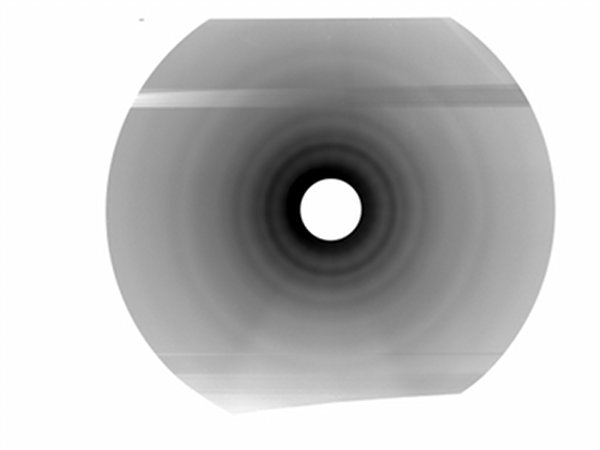
\includegraphics[width=12cm]{example}
\caption{An example of the raw data from the GED experiment, where an error ocurred during scanning, as can be seen from the irregular horizontal stripe. With the correct parameters, it may still be possible to extract useful information from the image.}
\label{example} 
\end{figure} 


 